\documentclass[11pt,a4paper]{article}
\usepackage[T1]{fontenc}
\usepackage[utf8]{inputenc}
\usepackage{lmodern}
\usepackage[margin=2cm]{geometry}
\usepackage{amsmath,amssymb}
\usepackage{booktabs,array,tabularx}
\usepackage{xcolor}
\usepackage{tikz}
\usetikzlibrary{arrows.meta,positioning,shapes.geometric,calc,fit}
\usepackage[ruled,vlined,linesnumbered]{algorithm2e}
\usepackage[colorlinks=true,linkcolor=blue!45!black,urlcolor=blue!45!black]{hyperref}
\newcommand{\code}[1]{\texttt{\detokenize{#1}}}
\newcolumntype{L}{>{\raggedright\arraybackslash}X}
\setlength{\parskip}{4pt}
\setlength{\parindent}{0pt}
\DeclareMathOperator*{\argmax}{arg\,max}
\DeclareMathOperator*{\argmin}{arg\,min}
\newcommand{\R}{\mathbb{R}}
\newcommand{\1}{\mathbf{1}}
\newcommand{\Reg}{\mathrm{Reg}}
\newcommand{\W}{\mathcal{W}}
\newcommand{\U}{\mathsf{U}}
\newcommand{\B}{\mathsf{B}}
\definecolor{navy}{RGB}{31,78,156}
\definecolor{leaf}{RGB}{46,139,87}
\definecolor{brick}{RGB}{192,57,43}
\tikzset{
  blk/.style={draw, thick, rounded corners=2pt, align=center, inner sep=5pt, fill=navy!6, font=\small},
  dat/.style={draw, thick, align=center, inner sep=5pt, fill=black!4, font=\small},
  dec/.style={diamond, draw, thick, aspect=2.4, align=center, inner sep=1.5pt, fill=brick!8, font=\small},
  res/.style={draw, thick, rounded corners=2pt, align=center, inner sep=5pt, fill=leaf!12, font=\small},
  arr/.style={-{Stealth[length=2.2mm]}, thick},
  lbl/.style={font=\scriptsize, fill=white, inner sep=1pt}
}
\newsavebox{\diagbox}
\newcommand{\fitdiagram}[1]{\sbox{\diagbox}{#1}\ifdim\wd\diagbox>\linewidth\resizebox{\linewidth}{!}{\usebox{\diagbox}}\else\usebox{\diagbox}\fi}
\SetKwProg{Fn}{function}{:}{end}
\SetKwFunction{Replay}{REPLAY}\SetKwFunction{Measure}{MEASURE}\SetKwFunction{Reg}{REG}\SetKwFunction{FitLeaf}{FIT\_LEAF}
\SetKwFunction{Grow}{GROW}\SetKwFunction{BestSplit}{BEST\_SPLIT}\SetKwFunction{Shortlist}{SHORTLIST}\SetKwFunction{Screen}{SCREEN}
\SetKwFunction{RefitAll}{REFIT\_ALL}\SetKwFunction{Prune}{PRUNE}\SetKwFunction{CheckPath}{CHECK\_PATH}\SetKwFunction{Visit}{VISIT}
\SetKwFunction{Scores}{SCORES}\SetKwFunction{Main}{MAIN}\SetKwFunction{Route}{ROUTE}
\SetKw{KwBreak}{break}\SetKw{KwSkip}{skip}\SetKw{KwAnd}{and}\SetKw{KwOr}{or}\SetKw{KwNone}{none}

\title{\vspace{-1.2cm}The SPO tree: the core algorithm, block by block\\[2pt]\large Growth and pruning as pseudo-code, as \code{spo_tree.py} runs them}
\author{}
\date{25 September 2026}

\begin{document}
\maketitle
\vspace{-0.8cm}

\section*{0. Notation and state}
\begin{tabularx}{\linewidth}{@{}>{\ttfamily}l L@{}}
\toprule
\normalfont symbol & meaning \\
\midrule
t = 1..T & decision dates, in time order ; $F$ = the first $75\%$ (fitting rows), $C$ = the last $25\%$ (checking rows)\\
x\_t, r\_t, \(\Sigma_t\) & features on date $t$ ; $h$-day simple returns of the $n$ assets (cash $=0$) ; $h$-day covariance from the past only\\
w*(c; u, \(\Sigma\)) & the optimizer: $\argmax_{w\in\W} c^\top w-f^\top|w-u|-\lambda w^\top\Sigma w$, $\W=\{0\le w_i\le\bar w,\ \1^\top w=1\}$, solved exactly because concave\\
utility(w; r, u, \(\Sigma\)) & $r^\top w-f^\top|w-u|-\lambda w^\top\Sigma w$\\
\(\U[t]\), \(\B[t]\) & training state, one row per date: holdings before decision $t$; hindsight utility from those holdings. Set by \Measure, frozen between two calls\\
leaf \(\ell\) = (node, rows, \(\omega\), depth) & node: score $\hat c_\ell\in[-b,b]^n$, mass $n_\ell$, regret sum $L_\ell$ ; rows: the dates reaching $\ell$; $\omega$: their weights\\
split node & feature $j$, threshold $\theta$, two children ; a soft node also holds thresholds $\theta_1<\dots<\theta_K$ and weights $\pi_k$\\
S & in-sample Sharpe ratio of the current tree's replayed path\\
\bottomrule
\end{tabularx}

\begin{sloppypar}
\textbf{Parameters of v1}: $\lambda=1$, 
$f=(3\,\mathrm{bp},0)$, 
$\bar w=1$, $b=10\%$, 
$m=\text{minimum number of rows in a leaf}=20$, 
$\varphi=\text{minimum fraction of rows from the parent in a leaf}=0.10$, 
$D=\text{maximum depth}=3$, 
shortlist splits (thresholds) $3$, 
$\varepsilon_R=\text{minimum regret loss improvement}=10^{-6}$, 
$\varepsilon_S=\text{minimum sharpe improvement}=0$, 
$k_p=\text{pruning hurdle}=2$, 
$D_p=\text{pruning depth}=1$, 
deciles $+$ refinement with $k=1$ (refinement hurdle: the refined threshold replaces the best decile only if its regret is lower by more than $k$ standard errors of the difference), 
$\kappa=\text{soft-split temperature}=0$.
\end{sloppypar}

\section{MAIN}
\begin{center}
\fitdiagram{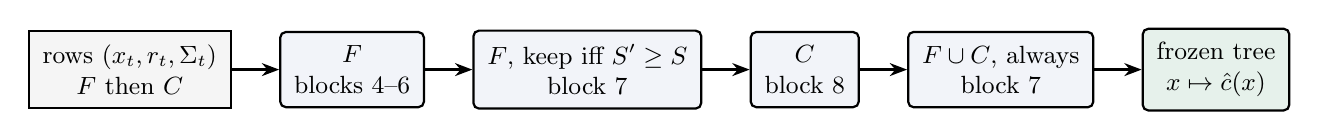
\begin{tikzpicture}[node distance=5mm and 6mm]
\node[dat] (rows) {rows $(x_t, r_t, \Sigma_t)$\\ $F$ then $C$};
\node[blk, right=of rows] (grow) {\Grow{$F$}\\ blocks 4--6};
\node[blk, right=of grow] (refit) {\RefitAll{$F$, keep iff $S'\ge S$}\\ block 7};
\node[blk, right=of refit] (prune) {\Prune{$C$}\\ block 8};
\node[blk, right=of prune] (final) {\RefitAll{$F\cup C$, always}\\ block 7};
\node[res, right=of final] (tree) {frozen tree\\ $x\mapsto\hat c(x)$};
\draw[arr] (rows)--(grow); \draw[arr] (grow)--(refit); \draw[arr] (refit)--(prune); \draw[arr] (prune)--(final); \draw[arr] (final)--(tree);
\end{tikzpicture}}
\end{center}
\begin{algorithm}[H]
\caption{\texttt{MAIN}: \texttt{SPOPortfolioTree.fit}}
\KwIn{rows $t=1..T$; $T_f=0.75T$; $F=\{1, ..., T_f\}$, $C=\{T_f+1, ..., T\}$}
root, leaves, path $\gets$ \Grow{$F$}\;
\RefitAll{leaves, path, rows $=F$, always $=$ false}\;
\Prune{root}\;
route all rows $F\cup C$ through the pruned tree; path $\gets$ \Replay{\Scores{leaves}, $F\cup C$, $u_1=\1/n$}; \Measure{path}\;
\RefitAll{leaves, path, rows $=F\cup C$, always $=$ true}\;
\KwOut{the tree; in use: $w_t=w^\star(\hat c(x_t);u_t,\Sigma_t)$ with the live holdings $u_t$}
\end{algorithm}

\section{REPLAY: the path, the fees, the row regrets}
Fees are computed here and nowhere else. One date:
\begin{center}
\fitdiagram{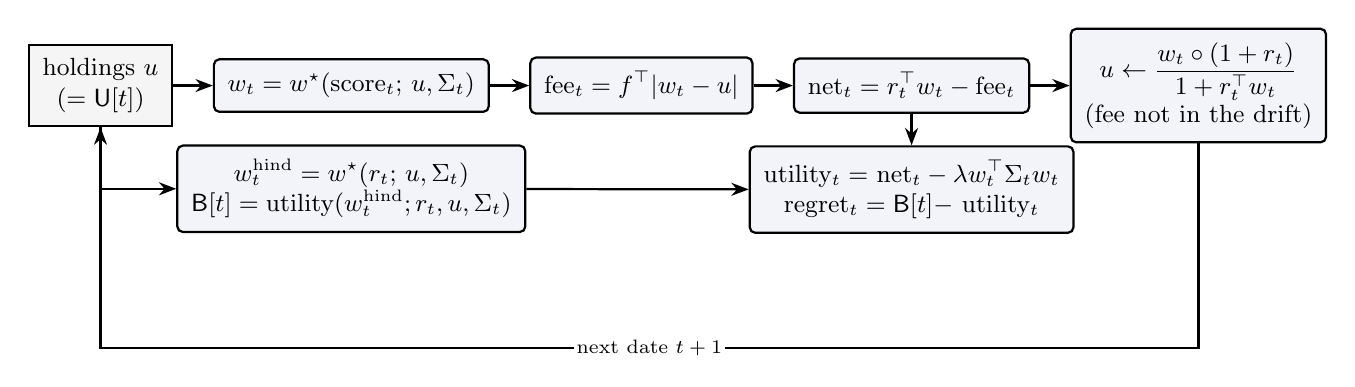
\begin{tikzpicture}[node distance=4mm and 5mm]
\node[dat] (u) {holdings $u$\\ ($=\U[t]$)};
\node[blk, right=of u] (opt) {$w_t=w^\star(\text{score}_t;\,u,\Sigma_t)$};
\node[blk, right=of opt] (fee) {fee$_t=f^\top|w_t-u|$};
\node[blk, right=of fee] (net) {net$_t=r_t^\top w_t-\text{fee}_t$};
\node[blk, right=of net] (drift) {$u\gets \dfrac{w_t\circ(1+r_t)}{1+r_t^\top w_t}$\\ (fee not in the drift)};
\node[blk, below=of opt] (hind) {$w^{\mathrm{hind}}_t=w^\star(r_t;\,u,\Sigma_t)$\\ $\B[t]=\text{utility}(w^{\mathrm{hind}}_t;r_t,u,\Sigma_t)$};
\node[blk, below=of net] (reg) {utility$_t=$ net$_t-\lambda w_t^\top\Sigma_tw_t$\\ regret$_t=\B[t]-$ utility$_t$};
\draw[arr] (u)--(opt); \draw[arr] (opt)--(fee); \draw[arr] (fee)--(net); \draw[arr] (net)--(drift);
\draw[arr] (u.south) |- (hind.west); \draw[arr] (hind)--(reg); \draw[arr] (net)--(reg);
\draw[arr] (drift.south) |- ++(0,-2.6) -| node[lbl, pos=0.25] {next date $t+1$} (u.south);
\end{tikzpicture}}
\end{center}
\begin{algorithm}[H]
\caption{\texttt{REPLAY}(scores, rows, $u_1$) (\texttt{replay\_path}) and \texttt{MEASURE}}
$u\gets u_1$\;
\For{$t$ in rows, in time order}{
  $\U[t]\gets u$;\quad $w_t\gets w^\star(\text{scores}_t;u,\Sigma_t)$\;
  fee$_t\gets f^\top|w_t-u|$;\quad net$_t\gets r_t^\top w_t-\text{fee}_t$\;
  $u\gets w_t\circ(1+r_t)\,/\,(1+r_t^\top w_t)$\;
}
utility$_t\gets r_t^\top w_t-\text{fee}_t-\lambda w_t^\top\Sigma_tw_t$;\quad $\B[t]\gets\text{utility}\big(w^\star(r_t;\U[t],\Sigma_t);r_t,\U[t],\Sigma_t\big)$;\quad regret$_t\gets\B[t]-\text{utility}_t$\;
$S\gets\mathrm{mean}(\text{net})/\mathrm{std}(\text{net})$ \tcp*{$0$ if net $\equiv0$}
\Return path $=(\U,w,\text{net},\text{regret},S,\ \text{final }u)$\;
\BlankLine
\Fn{\Measure{path}}{$\U\gets$ path.$\U$;\quad $\B\gets$ path.utility $+$ path.regret;\quad $S\gets$ path.$S$ \tcp*{holdings frozen from here}}
\end{algorithm}

\section{The row regret and the score search of a leaf}
\begin{algorithm}[H]
\caption{\texttt{REG}($c$, $t$) (\texttt{\_regret\_rows}) and \texttt{FIT\_LEAF}(rows, $\omega$, fallback) (\texttt{\_fit\_leaf})}
\Fn{\Reg{$c$, $t$}}{
  $w\gets w^\star(c;\U[t],\Sigma_t)$;\quad \Return $\max\big(\B[t]-\text{utility}(w;r_t,\U[t],\Sigma_t),\,0\big)$ \tcp*{abort if $<-10^{-6}$}
}
$L(c)\;:=\;\sum_{t\in\text{rows}}\omega_t\,\Reg(c,t)$ \tcp*{leaf regret of a score vector}
\Fn{\FitLeaf{rows, $\omega$, fallback}}{
  $c\gets\mathrm{clip}\big(\sum_t\omega_tr_t/\sum_t\omega_t,\ -b,\ b\big)$ \tcp*{start: the weighted mean return}
  \If{fallback given \KwAnd $L(\text{fallback})<L(c)$}{$c\gets$ fallback}
  radius $\gets2b$\;
  \For{pass $=1,2,3$}{
    \For{coord in (asset, cash)}{
      grid $\gets$ 7 equally spaced values in $[c_{\text{coord}}-\text{radius},\,c_{\text{coord}}+\text{radius}]\cap[-b,b]$ \tcp*{pass 1: all of $[-b,b]$}
      $c_{\text{coord}}\gets$ the grid value with the smallest $L$, if strictly smaller than the current $L(c)$\;
    }
    radius $\gets$ radius$/6$\;
  }
  \Return node$(\hat c=c,\ n=\sum\omega,\ L=L(c))$\;
}
\end{algorithm}
Cost: $2+3\cdot7\cdot n$ evaluations of $L$, each one vectorised optimizer call over the leaf's rows. Only score differences matter, so the cash coordinate is redundant; cash is reported as $0$.

\section{GROW}
\begin{algorithm}[H]
\caption{\texttt{GROW}($F$) (\texttt{\_grow})}
$\U[t]\gets\1/n$, $\B[t]\gets\text{utility}\big(w^\star(r_t;\1/n,\Sigma_t);r_t,\1/n,\Sigma_t\big)$ for all $t\in F$ \tcp*{convention: no path exists yet}
root $\gets$ \FitLeaf{$F$, $\omega\equiv1$, none};\quad leaves $\gets[(\text{root},F,\1,\text{depth }0)]$\;
path $\gets$ \Replay{\Scores{leaves}, $F$, $\1/n$};\quad \Measure{path}\;
\While{true}{
  result $\gets$ \BestSplit{leaves, $S$} \tcp*{block 5}
  \If{result $=$ \KwNone}{\KwBreak}
  leaves $\gets$ leaves $-\{\ell\}+\{\text{left child},\text{right child}\}$; node of $\ell$ becomes a split node $(j,\theta)$\;
  path $\gets$ result.path;\quad \Measure{path} \tcp*{new holdings, new $S$; children keep the rows of step 5}
}
\Return root, leaves, path\;
\end{algorithm}
\Scores{leaves}: the per-row score matrix, row $t$ $=\sum_\ell\omega_{t\ell}\hat c_\ell$ (one leaf per row with plain splits).

\section{BEST\_SPLIT: one round}
\begin{center}
\fitdiagram{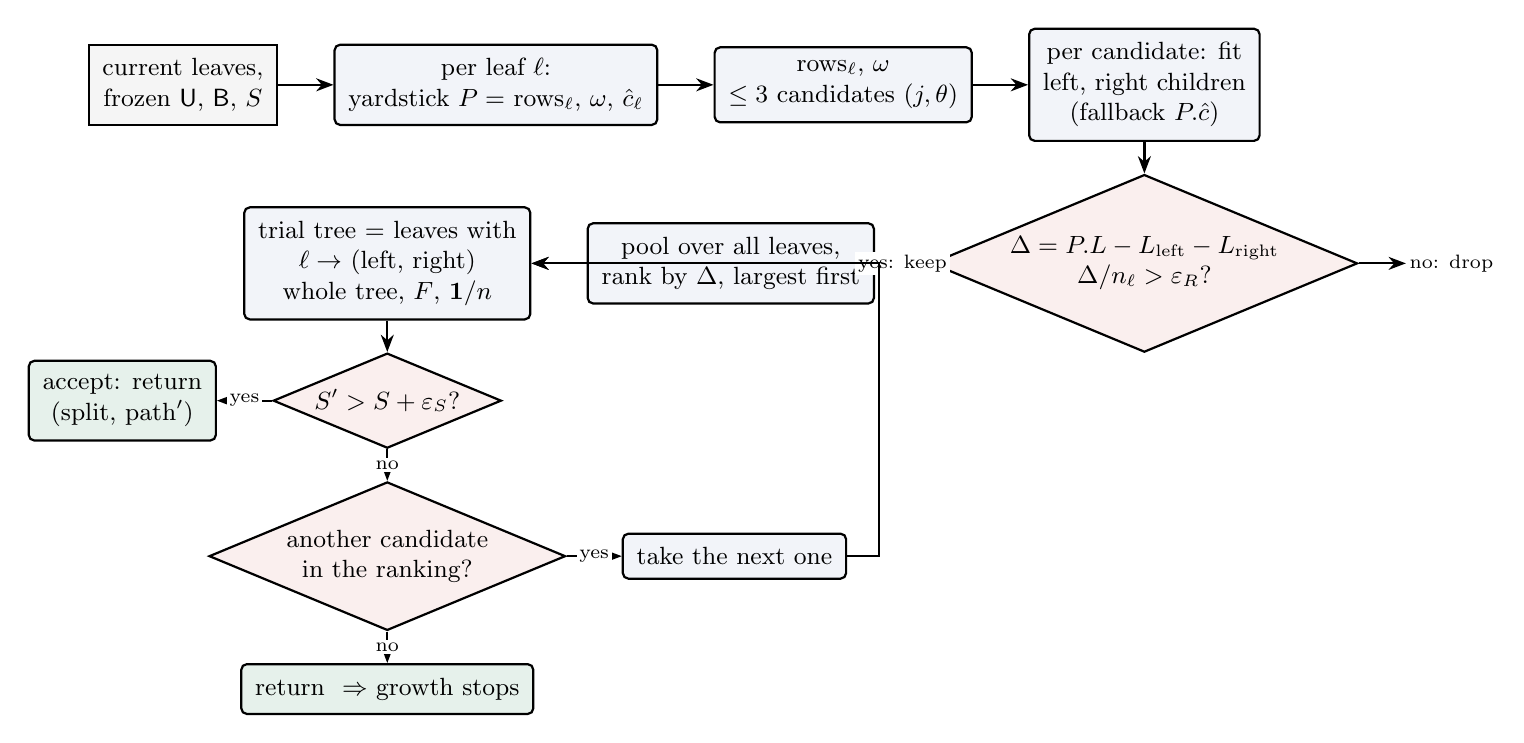
\begin{tikzpicture}[node distance=4mm and 7mm]
\node[dat] (leaves) {current leaves,\\ frozen $\U$, $\B$, $S$};
\node[blk, right=of leaves] (yard) {per leaf $\ell$:\\ yardstick $P=$ \FitLeaf{rows$_\ell$, $\omega$, $\hat c_\ell$}};
\node[blk, right=of yard] (cand) {\Shortlist{rows$_\ell$, $\omega$}\\ $\le3$ candidates $(j,\theta)$};
\node[blk, right=of cand] (child) {per candidate: fit\\ left, right children\\ (fallback $P.\hat c$)};
\node[dec, below=of child] (gate1) {$\Delta=P.L-L_{\text{left}}-L_{\text{right}}$\\ $\Delta/n_\ell>\varepsilon_R$?};
\node[blk, left=of gate1] (pool) {pool over all leaves,\\ rank by $\Delta$, largest first};
\node[blk, left=of pool] (trial) {trial tree $=$ leaves with\\ $\ell\to$ (left, right)\\ \Replay{whole tree, $F$, $\1/n$}};
\node[dec, below=of trial] (gate2) {$S'>S+\varepsilon_S$?};
\node[res, left=of gate2] (acc) {accept: return\\ (split, path$'$)};
\node[dec, below=of gate2] (more) {another candidate\\ in the ranking?};
\node[blk, right=of more] (next) {take the next one};
\node[res, below=of more] (none) {return \KwNone\ $\Rightarrow$ growth stops};
\draw[arr] (leaves)--(yard); \draw[arr] (yard)--(cand); \draw[arr] (cand)--(child); \draw[arr] (child)--(gate1);
\draw[arr] (gate1)--node[lbl]{yes: keep}(pool); \draw[arr] (gate1.east) -- ++(6mm,0) node[lbl, right]{no: drop};
\draw[arr] (pool)--(trial); \draw[arr] (trial)--(gate2);
\draw[arr] (gate2)--node[lbl]{yes}(acc); \draw[arr] (gate2)--node[lbl]{no}(more);
\draw[arr] (more)--node[lbl]{yes}(next); \draw[arr] (more)--node[lbl]{no}(none);
\draw[arr] (next.east) -- ++(4mm,0) |- (trial.east);
\end{tikzpicture}}
\end{center}
\begin{algorithm}[H]
\caption{\texttt{BEST\_SPLIT}(leaves, $S$) (\texttt{\_best\_split})}
cand $\gets[\,]$\;
\ForEach{leaf $\ell=(\text{node},\text{rows},\omega,\text{depth})$}{
  \If{depth $\ge D$ \KwOr $\sum\omega<2m_\ast$, $m_\ast=\max(m,\lceil\varphi\sum\omega\rceil)$}{\KwSkip}
  $P\gets$ \FitLeaf{rows, $\omega$, node.$\hat c$} \tcp*{same rows, current $\U$: the yardstick; never written into the tree}
  \ForEach{$(j,\theta)$ in \Shortlist{rows, $\omega$}}{
    left $\gets\{t\in\text{rows}: x_{tj}\le\theta\}$;\quad right $\gets$ rows $\setminus$ left\;
    $\text{Lc}\gets$ \FitLeaf{left, $\omega$, $P.\hat c$};\quad $\text{Rc}\gets$ \FitLeaf{right, $\omega$, $P.\hat c$}\;
    $\Delta\gets P.L-\text{Lc}.L-\text{Rc}.L$\;
    \If{$\Delta/\sum\omega>\varepsilon_R$}{cand $\gets$ cand $+(\Delta,\ell,j,\theta,\text{Lc},\text{Rc})$ \tcp*{regret gate: local, $\U$ frozen}}
  }
}
sort cand by $\Delta$, largest first \tcp*{SPOT's criterion, over all leaves}
\ForEach{$(\Delta,\ell,j,\theta,\text{Lc},\text{Rc})$ in cand}{
  trial $\gets$ leaves with $\ell$ replaced by $(\text{Lc},\text{left rows}),(\text{Rc},\text{right rows})$ \tcp*{other leaves unchanged}
  path$'\gets$ \Replay{\Scores{trial}, $F$, $\1/n$} \tcp*{whole tree, whole fitting period, fees included}
  \If{path$'$.$S>S+\varepsilon_S$}{\Return (split, path$'$) \tcp*{Sharpe gate: in-sample; one acceptance per round}}
}
\Return \KwNone\;
\end{algorithm}
With plain splits the memberships are $0/1$: left rows get $\omega$, right rows get $\omega$. With soft splits ($\kappa>0$) a row goes left with weight $\mu(x)=\sum_{k:\theta_k\ge x}\pi_k$ and right with $1-\mu(x)$, and a row can be in both children.

\section{SHORTLIST and SCREEN: the candidates of one leaf}
\begin{algorithm}[H]
\caption{\texttt{SHORTLIST}(rows, $\omega$) (\texttt{\_shortlist}), v1 settings; the soft variant in the last lines}
$m_\ast\gets\max(m,\lceil\varphi\sum\omega\rceil)$;\quad screened $\gets[\,]$\;
\ForEach{feature $j$}{
  $\Theta\gets$ midpoints of consecutive distinct values of $x_{\cdot j}$ on rows with mass $\ge m_\ast$ on each side \tcp*{plain candidates $\theta_{(1)}<\dots<\theta_{(K)}$}
  \If{deciles}{$\Theta\gets\Theta[\mathrm{round}(q\,(K-1))]$ for $q=0.1,\dots,0.9$ \tcp*{quantiles by rank among the admissible thresholds}}
  $Q,\ \text{per\_row}\gets$ \Screen{rows, $\omega$, $x_{\cdot j}$, $\Theta$}\;
  \If{refinement}{
    $\theta_\circ\gets\argmin_\Theta Q$;\quad $W\gets$ plain thresholds strictly between the two elements of $\Theta$ neighbouring $\theta_\circ$\;
    $Q_W,\ \text{per\_row}_W\gets$ \Screen{rows, $\omega$, $x_{\cdot j}$, $W$};\quad $\theta_\bullet\gets\argmin_WQ_W$\;
    se $\gets\sqrt{|\text{rows}|}\cdot\mathrm{std}_t\big(\text{per\_row}_W[\theta_\bullet]-\text{per\_row}[\theta_\circ]\big)$\;
    \If{$Q(\theta_\circ)-Q_W(\theta_\bullet)>k\cdot\mathrm{se}$}{replace $\theta_\circ$ by $\theta_\bullet$ in $\Theta$ (and its $Q$)}
  }
  \eIf{$\kappa=0$ (plain)}{screened $\gets$ screened $+\{(Q(\theta),j,\theta):\theta\in\Theta\}$}{
    $z_k\gets\big(Q(\theta_k)-\min_lQ(\theta_l)\big)/\mathrm{se}_k$;\quad $\pi_k\propto e^{-z_k/\kappa}$ (or $e^{-z_k^2/2\kappa^2}$);\quad screened $\gets$ screened $+\{(\min Q,j,\Theta,\pi)\}$ \tcp*{one soft split per feature}
  }
}
\Return the 3 entries of screened with the smallest $Q$\;
\BlankLine
\Fn{\Screen{rows, $\omega$, values, $\Theta$}}{
  \ForEach{$\theta\in\Theta$}{
    \ForEach{side in (values $\le\theta$, values $>\theta$)}{
      $c_{\text{side}}\gets\mathrm{clip}(\text{weighted mean of }r_t\text{ on the side},\pm b)$;\quad regret$_t\gets\omega_t\Reg(c_{\text{side}},t)$ for $t$ on the side\;
    }
    $Q(\theta)\gets\sum_t\text{regret}_t$;\quad per\_row$[\theta]\gets(\text{regret}_t)_t$\;
  }
  \Return $Q$, per\_row\;
}
\end{algorithm}

\section{REFIT\_ALL}
\begin{algorithm}[H]
\caption{\texttt{REFIT\_ALL}(leaves, path, rows, always) (\texttt{\_refit\_leaves})}
\ForEach{leaf $\ell$}{$\hat c'_\ell\gets$ \FitLeaf{rows$_\ell$, $\omega_\ell$, $\hat c_\ell$} \tcp*{from the current $\U$ (the path of the final tree)}}
path$'\gets$ \Replay{scores with $\hat c'$, rows, $\1/n$}\;
\If{always \KwOr path$'$.$S\ge$ path.$S$}{write every $\hat c'_\ell$ into its leaf \tcp*{all or nothing}}
\end{algorithm}
Step 4 (after growth): rows $=F$, kept only if $S$ does not fall. Step 6 (after pruning): rows $=F\cup C$ routed through the pruned tree, \Measure\ first, always kept: the scores it replaces never saw $C$.

\section{PRUNE: bottom-up on the checking rows}
\begin{center}
\fitdiagram{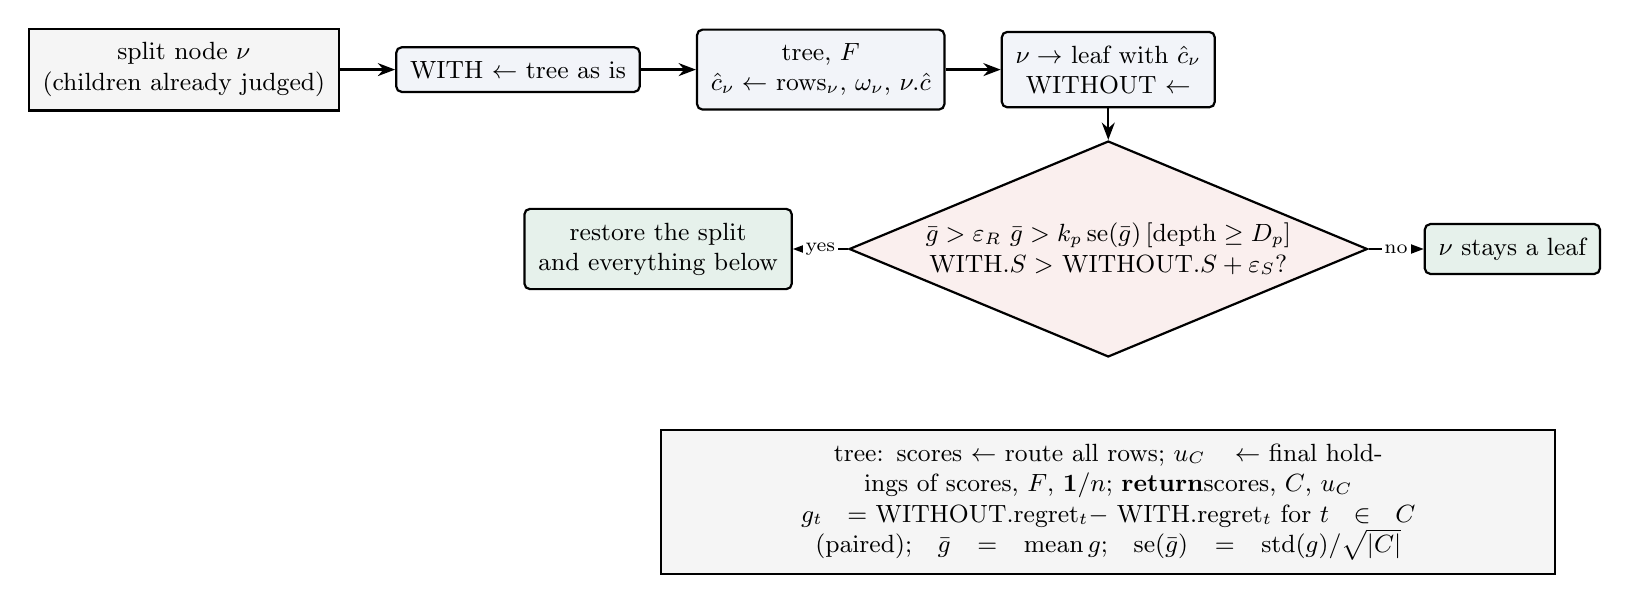
\begin{tikzpicture}[node distance=4mm and 7mm]
\node[dat] (nu) {split node $\nu$\\ (children already judged)};
\node[blk, right=of nu] (with) {WITH $\gets$ \CheckPath{tree as is}};
\node[blk, right=of with] (fit) {\Measure{\Replay{tree, $F$}}\\ $\hat c_\nu\gets$ \FitLeaf{rows$_\nu$, $\omega_\nu$, $\nu.\hat c$}};
\node[blk, right=of fit] (without) {$\nu\to$ leaf with $\hat c_\nu$\\ WITHOUT $\gets$ \CheckPath{}};
\node[dec, below=of without] (test) {$\bar g>\varepsilon_R$ \KwAnd $\bar g>k_p\,\mathrm{se}(\bar g)\,[\text{depth}\ge D_p]$\\ \KwAnd WITH.$S>$ WITHOUT.$S+\varepsilon_S$?};
\node[res, left=of test] (keep) {restore the split\\ and everything below};
\node[res, right=of test] (rm) {$\nu$ stays a leaf};
\draw[arr] (nu)--(with); \draw[arr] (with)--(fit); \draw[arr] (fit)--(without); \draw[arr] (without)--(test);
\draw[arr] (test)--node[lbl]{yes}(keep); \draw[arr] (test)--node[lbl]{no}(rm);
\node[dat, below=9mm of test, text width=11cm] (cp) {\CheckPath{tree}: scores $\gets$ route all rows; $u_C\gets$ final holdings of \Replay{scores, $F$, $\1/n$}; \Return \Replay{scores, $C$, $u_C$}\\ $g_t=$ WITHOUT.regret$_t-$ WITH.regret$_t$ for $t\in C$ (paired);\quad $\bar g=\mathrm{mean}\,g$;\quad $\mathrm{se}(\bar g)=\mathrm{std}(g)/\sqrt{|C|}$};
\end{tikzpicture}}
\end{center}
\begin{algorithm}[H]
\caption{\texttt{PRUNE}(root) (\texttt{\_prune})}
\Fn{\Visit{$\nu$, rows$_\nu$, $\omega_\nu$, depth}}{
  \If{$\nu$ is a leaf}{\Return}
  \Visit{left child, its rows, its weights, depth$+1$};\quad \Visit{right child, \dots} \tcp*{children first}
  WITH $\gets$ \CheckPath{tree as it is}\;
  \Measure{\Replay{\Scores{current leaves}, $F$, $\1/n$}} \tcp*{holdings for the leaf fit}
  $\hat c_\nu\gets$ \FitLeaf{rows$_\nu$, $\omega_\nu$, $\nu.\hat c$};\quad make $\nu$ a leaf with $\hat c_\nu$, detaching the subtree\;
  WITHOUT $\gets$ \CheckPath{tree with $\nu$ as a leaf}\;
  $g_t\gets$ WITHOUT.regret$_t-$ WITH.regret$_t$ for $t\in C$;\quad $\bar g\gets\mathrm{mean}(g)$;\quad se $\gets\mathrm{std}(g)/\sqrt{|C|}$\;
  keep $\gets\bar g>\varepsilon_R$ \KwAnd $\bar g>(k_p\,\mathrm{se}$ if depth $\ge D_p$ else $0)$ \KwAnd WITH.$S>$ WITHOUT.$S+\varepsilon_S$\;
  \eIf{keep}{restore the split and its subtree}{$\nu$ stays a leaf with $\hat c_\nu$}
}
\Visit{root, $F$, $\1$, 0}\;
\BlankLine
\Fn{\CheckPath{tree}}{
  scores $\gets$ \Route{all rows $F\cup C$}\;
  $u_C\gets$ final holdings of \Replay{scores$_F$, $F$, $\1/n$};\quad \Return \Replay{scores$_C$, $C$, $u_C$} \tcp*{fees included; regrets and $S$ on $C$ only}
}
\end{algorithm}
With $k_p=2$, $D_p=1$: the root split is judged by the plain rule ($\bar g>\varepsilon_R$ and the Sharpe test); every deeper split must beat two standard errors. A split no checking row reaches has $\bar g=0$ and is removed.

\section{Where each quantity lives, and the two facts to remember}
\begin{tabularx}{\linewidth}{@{}l L L@{}}
\toprule
per date $t$ & $\U[t]$, $\B[t]$, $w_t$, net$_t$, regret$_t$ & written by \Replay/\Measure; read by \Reg; never stored in a node\\
per leaf $\ell$ & $\hat c_\ell$, $n_\ell$, $L_\ell$, rows$_\ell$, $\omega_\ell$ & rows and $\omega$ are training state; the frozen tree keeps $\hat c_\ell$ and $n_\ell$\\
per split node & $j$, $\theta$ (soft: $\theta_k$, $\pi_k$, spread), children & no score in use, no holdings\\
per round & $S$, the ranking of candidates & recomputed from scratch each round\\
\bottomrule
\end{tabularx}
\begin{itemize}\setlength{\itemsep}{1pt}
\item \textbf{Fees enter only through \Replay}: fee$_t=f^\top|w_t-u|$ on the path. The regret sees them through $\U[t]$ (frozen for a round) and through $|w-\U[t]|$ inside the utility.
\item \textbf{Holdings do not move while a candidate split is judged}: the regret gate compares one score against two scores on the same rows from the same $\U$. The candidate's true path appears only in the Sharpe gate's replay, and becomes the new $\U$ through \Measure\ when the split is accepted.
\end{itemize}

\section*{Code map}
\begin{tabularx}{\linewidth}{@{}>{\ttfamily}l L@{}}
\toprule
\normalfont block & function in \code{code/spo_tree.py} \\
\midrule
MAIN & \code{SPOPortfolioTree.fit}\\
REPLAY, fees, drift & \code{replay_path}, \code{_trade}; \code{SPOPortfolioTree._replay}, \code{_measure_from}\\
REG, FIT\_LEAF & \code{_regret_rows}, \code{_score_prediction}, \code{_fit_leaf}\\
GROW, BEST\_SPLIT & \code{_grow}, \code{_best_split}, \code{_scores}, \code{_leaves}\\
SHORTLIST, SCREEN & \code{_shortlist}, \code{_screen}, \code{_thresholds}, \code{_standard_error}, \code{_membership_of}\\
REFIT\_ALL & \code{_refit_leaves}\\
PRUNE, CHECK\_PATH & \code{_prune} (inner \code{visit}, \code{checking_path})\\
optimizer & \code{PortfolioOptimizer.solve} ($5^n$ enumeration), \code{PortfolioOptimizer.utility}\\
\bottomrule
\end{tabularx}
\end{document}
